\documentclass[pstricks,serif, 10pt]{beamer}

\usetheme{JuanLesPins}
\useinnertheme{rounded}
\useoutertheme{infolines}
%\usecolortheme{fly}
\usefonttheme[onlymath, stillsansserifmath]{serif}


\usepackage[utf8]{inputenc}
\usepackage{amsthm}
\usepackage[spanish]{babel}
\usepackage{alltt}
\usepackage{colortbl}
\usepackage{enumerate}
\usepackage{pdfpages}
\usepackage{multimedia}
\setbeamercovered{transparent}
\usepackage{tabulary}
\usepackage{graphicx}

\title[Comunicación SoC-SystemC]{Modeling I$^2$C Communication Between SoCs with SystemC-AMS}
\author[Martínez, Zapata]{David Ricardo Martínez Hernández\\
			   Sergio Andrés Zapata Palomino}
\institute[UNAL]{Universidad Nacional de Colombia}
\date[06/12/2013]{Bogotá 6 de diciembre 2013}

\begin{document}
\begin{frame}
  \titlepage
\end{frame}

\begin{frame}[allowframebreak]
 \frametitle{Tabla de Contenidos}
 %\begin{block}
 \tableofcontents
 %\end{block}
\end{frame}

\section{Introducción}
\subsection{SystemC-AMS}
\begin{frame}[allowframebreak]
 \frametitle{SystemC-AMS}
 \begin{itemize}
  \item Sistemas embebidos, combinación elementos digitales y análogos. 
  \item VHDL-AMS y SystemC.
  \item SystemC-AMS.
 \end{itemize}
\end{frame}

\section[I$^2$C]{Protocolo I$^2$C}
\subsection{Transmisión}
\begin{frame}[allowframebreak]
 \frametitle{Transmisión}
 \begin{block}{Protocolo I$^2$C}
 \begin{itemize}
  \item Frecuencia de transferencia de $100\, Kbits/s$.
  \item Modo de direccionamiento de $7\, bits$.
 \end{itemize}
 \end{block}

  \begin{itemize}
   \item Transferencias inician cuando hay flanco de bajada en el SDA mientras el SCL está en alto.
   \item Transferencias terminan cuando hay una flanco de subida en el SDA mientras el SCL  está en alto.
  \end{itemize}
  \begin{figure}[H]
  \centering
    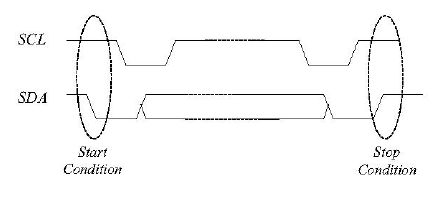
\includegraphics[scale=0.35]{trans.png}
      \caption{Inicio y terminación de una transmisión.}
	\label{fig1}
\end{figure}
\end{frame}

\subsection{Validación}
\begin{frame}[allowframebreak]
 \frametitle{Validación}
  \begin{itemize}
   \item La información transmitida es considerada válida cuando SCL se mantiene en estado alto.
  \end{itemize}
  \begin{figure}[H]
  \centering
    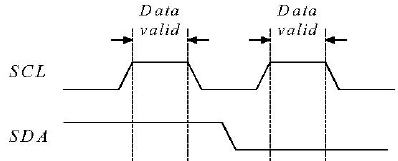
\includegraphics[scale=0.35]{val.png}
      \caption{Validación de datos.}
	\label{fig2}
\end{figure}
\end{frame}

\subsection{Comunicación Multimaster}
\begin{frame}[allowframebreak]
 \frametitle{Comunicación Multimaster}
  \begin{itemize}
   \item Arbitraje en la linea SDA.
  \end{itemize}
  \begin{figure}[H]
  \centering
    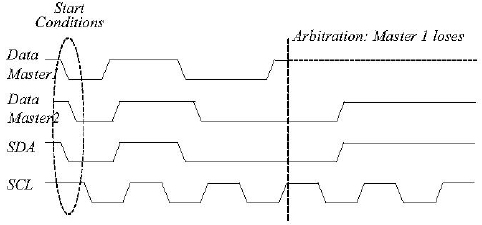
\includegraphics[scale=0.35]{com.png}
      \caption{Procedimiento de arbitraje con 2 masters.}
	\label{fig3}
\end{figure}
\end{frame}

\section[Controlador]{Controlador para la arquitectura del bus I$^2$C}
\subsection[Arquitectura y Modelamiento]{Arquitectura General y Lenguaje de Modelamiento}
\begin{frame}
 \frametitle{Arquitectura General y Lenguaje de Modelamiento}
 \begin{itemize}
  \item Inventado para proveer comunicación en un bus bi-direccional de dos clables, usado en sensores, micotrocontroladores, LCD.
  \item Compatible con los estandares manejados por Philips.
  \item Detección de uso de bus.
 \end{itemize}
 \begin{figure}[H]
  \centering
    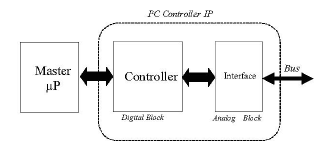
\includegraphics[scale=0.5]{general.png}
      \caption{Arquitectura de bloque.}
	\label{fig4}
\end{figure}
\end{frame}

\subsection{Arquitectura Digital de Bloques}
\begin{frame}
  \frametitle{Bloques de la Arquitectura Digital}
  \begin{itemize}
   \item Hay una lista FIFO que guarda las ordenes que vienen del procesador.
   \item Esas ordenes que provienen del micoprocesador se convierten en secuencias detalladas usando el protocolo I$^2$C.
   \item Mediante un generador de señales se manejan las líneas del bus SCL y DSA.
  \end{itemize}
 \begin{figure}[H]
  \centering
    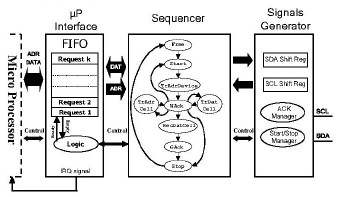
\includegraphics[scale=0.5]{digital.png}
      \caption{Arquitectura digital de bloques.}
	\label{fig4}
\end{figure}  
\end{frame}

\subsection{Bloques Analógicos}
\begin{frame}
 \frametitle{Bloques Analógicos}
 \begin{itemize}
  \item Puede tener salidas de tipo Colector-Abierto o de Drenador-Abierto.
  \item El capacitor se utiliza para controlar el tiempo de salida y de bajada para la señal SDA.
 \end{itemize}
 \begin{figure}[H]
  \centering
    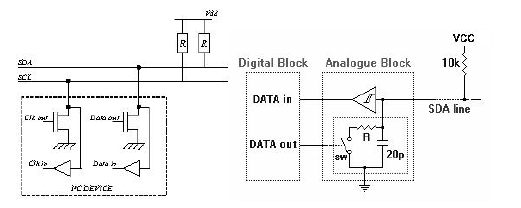
\includegraphics[scale=0.6]{ana.png}
      \caption{Arquitectura análoga de bloques.}
	\label{fig5}
\end{figure}  
\end{frame}

\section[Simulación]{Simulación del Controlador I$^2$C}
\subsection[Micro-Controlador]{Simulación de un Micro-Controlador del Nodo}
\begin{frame}
 \frametitle{Simulación de un Micro-Controlador del Nodo}
 \begin{figure}[H]
  \centering
    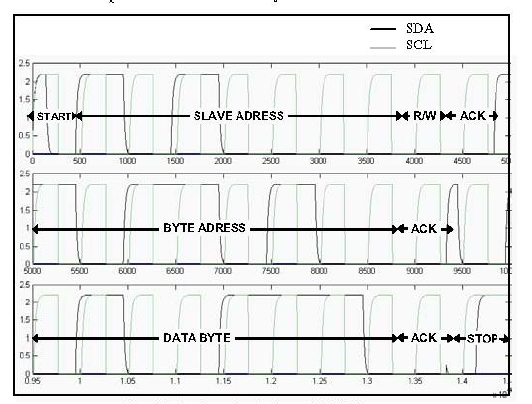
\includegraphics[scale=0.5]{sim1.png}
      \caption{Simulación análoga con master 8051.}
	\label{fig5}
\end{figure}  
\end{frame}

\subsection[SoC]{Simulación de una SoC del Nodo}
\begin{frame}
 \frametitle{Simulación de una SoC del Nodo}
 \begin{figure}[H]
  \centering
    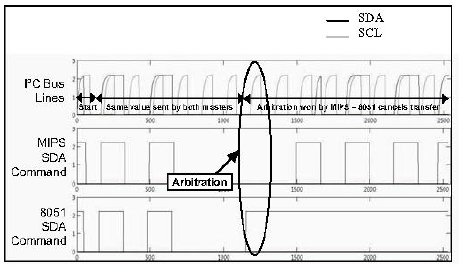
\includegraphics[scale=0.6]{sim2.png}
      \caption{Multimaster Arbitraje.}
	\label{fig5}
\end{figure}  
\end{frame}

\subsection[Rendimiento]{Simulación Rendimiento}
\begin{frame}
 \frametitle{Simulación Rendimiento}
 \begin{figure}[H]
  \centering
    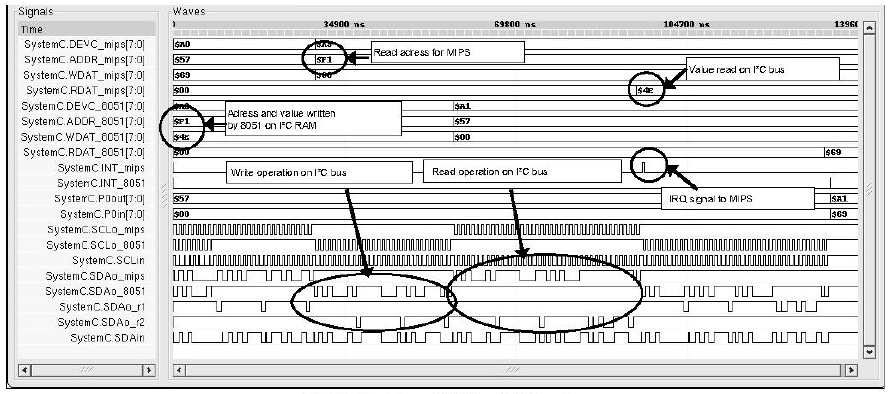
\includegraphics[scale=0.39]{sim3.png}
      \caption{Simulación con master 8051 y mastert MIPS.}
	\label{fig5}
\end{figure}  
\end{frame}

\section{Bibliografía}
\begin{frame}
  \frametitle{Bibliografía}    
  \begin{thebibliography}{10}    
  %\beamertemplatebookbibitems
  %\bibitem{Autor1990}
  %  A.~Autor.
  %  \newblock {\em Einf¸hrung in das Prsentationswesen}.
   % \newblock Klein-Verlag, 1990.
  \beamertemplatearticlebibitems
  \bibitem{articule1}
    Mohamad Alassir, Julien Denoulet, Olivier Romain, Patrick Garda.
    \newblock {\em Modelado de Comunicación I$^2$C entre SoCs con SystemC-AMS}.
    \newblock{Universite Pierre et Marie Curie - Paris 6 - EA2385, 3 Rue Galilee - Boite Courrier 252 94200 - Ivry sur Seine, France.}
  \end{thebibliography}
\end{frame}
\end{document}
